\chapter{Post Processing}

% Why post processing? Cool effects that can easily be applied to any
% project and reused.

In the previous sections we've had to use geometry to help us create
the landscape, sky and rendering it to the screen. Now we will turn to
screen space effects, which doesn't rely on geometry, but will instead
use the final color image and the depth buffer to create the
effects. Depth of field, motion blur and a screenwide glow are all
effects that can easily be produced through post processing and there
are many more.

% Easy to use important. Should handle most of the setup

We will try to create a general framework inside OpenEngine that can
handle most effects with the programmer having to do as little setup
as possible. It should also be possible to layer post processing
effects on top of each other, for example to combine a cel shader with
edge detection or optimizing blurring by using a technique called
separable convolution.

\section{Structure}

In this section we will first outline the new scene node called post
process node and how it will help the programmer setup post
processing. Then we will discuss the specifics of rendering the scene,
applying the post process effect to it and how we eventually chose to
structure the rendering.

\subsection*{Post Process Node}

The post process node will apply a fragment program to manipulate the
image rendered while visiting subnodes. Therefore it of course
contains an IShaderResourcePtr that points to the effect. It also
contains a pointer to an OpenEngine FrameBuffer, which the scene is
rendered to, and another FrameBuffer where the scene with the effect
is rendered into. Why the effect is not simply rendered directly to
the backbuffer (or previous frame buffer in case of chained effects)
is explained in the Rendering subsection. The postprocess node also
has a list of \class{ITexture2DPtr's} where the final image can be stored
after the effect has been applied, this is useful for some
implementations of motion blur, that relies on the previous image
being availible.

In order to allow users of the PostProcessNode to focus on writing
their effects, the node will handle most of the setup as long as a few
naming conventions are followed. If a uniform named \textit{depth} is
detected then the subscenes depth texture will be bound to this
uniform. Similarly if \textit{imageN}, where \textit{N} is any
integer, is seen, then the FrameBuffer's \textit{N}'th color
attachment will be bound to that uniform. The same goes for the final
image and the uniform name \textit{finalImageN}. The node can also
decide to improve performance by not copying the final image, if this
isn't needed. Of course the previous image doesn't make sense in the
very first rendering, so when initialized the node binds the
not-processed scene image as the final image, and then after the first
frame it switches to the final image. And finally, if needed the node
will pass the time to the shader.

All of this has allowed us to cut back on doing setup and spend our
time writing cool and fun effects.

\subsection*{Rendering}

% render to a framebuffer

The first thing that needs to be done before switching to the new
framebuffer is to save the old state. This means saving the name of
the old framebuffer and the dimensions of the viewport.

Once the state has been saved we set the viewport size to the one
specified in the nodes framebuffer and proceed to bind the framebuffer
and clear the color and depth. The subscene is then rendered to the
framebuffer.

% Apply the effect with depth testing set to always

When the scene has been rendered we bind the previous frame buffer and
set OpenGL's depth function to always let fragments pass. We can do
this since we're applying a post process to the entire image and it's
cheaper performance wise than clearing the depth buffer each pass. The
depth test couldn't simply be disabled as that would disable writes to
the depth buffer aswell, and we are interested in keeping the depth
values or maybe modifying them through a post process.

With the previous framebuffer bound, we apply the post process shader
and render a rectangle to the screen. The rectangle is simply drawn
from (-1,-1) to (1,1). If no matrices are applied to these vertices,
then the rectangle will cover the screen.

% Store the final image

If our post process effect relies on the final image from the last
rendering, then now is the time to save it. However first we have to
initialize the final framebuffer and attach the final color images to
the post process shader. Then we blit the image with it's effect into
the final image framebuffer, rescaling the image if the source and
destination rectangles are not of the same size.

% Allows multiple postprocess nodes

\section{Post Pocess Effect}

In this section we will take to a short look at some of the different
post process efects that we have created.

\subsection{Motion Blur}

While motion blurring may not be critical to outdoor environments,
many projects still benefit from it. Therefore one of the criteria
to the post process node was that it would allow an easy motion blur
implementation for existing and future open engine projects.

Motion blurring can be done in several ways. The simplest way
conceptually is to store the last $n$ images and then blend them
together. This creates a nice blurring effect across the last few
frames. The problem is that we then need to store the last few frames
in memory, giving us a memory overhead of 8-16 textures. Another
problem is that the blurring is framerate dependent, so low framerates
will make the blurring excessive, while high framerates will make it
non existent.

Another approach was proposed in GPU Gems 3, where the previous
ViewProjection matrix is used to calculate the previous position of a
fragment and then accumulate the colors between the current and
previous position. This approach however only creates blurring if the
camera is moved. A car that drives past the camera will crystal
clear. Another problem is that the shader becomes quite complex and
timeconsuming.

The algorithm that we settled on is a ghosting motion blur and
combines a low memory footprint with a fast shader. We use an
acuumulation texture for storing all the previous images blended
together, and then blend that together with the current image. That
way the effect from old images will tend toward 0 and the motion
blurring will produce nice looking blurred 'tails' on moving
objects. Ofcourse since we can only blur between rendered frames, a
fast turning camera will produce artefacts.

The result can be seen in \reffig{fig:motionblur}

\begin{figure}
  \label{fig:motionblur}
  \centering
  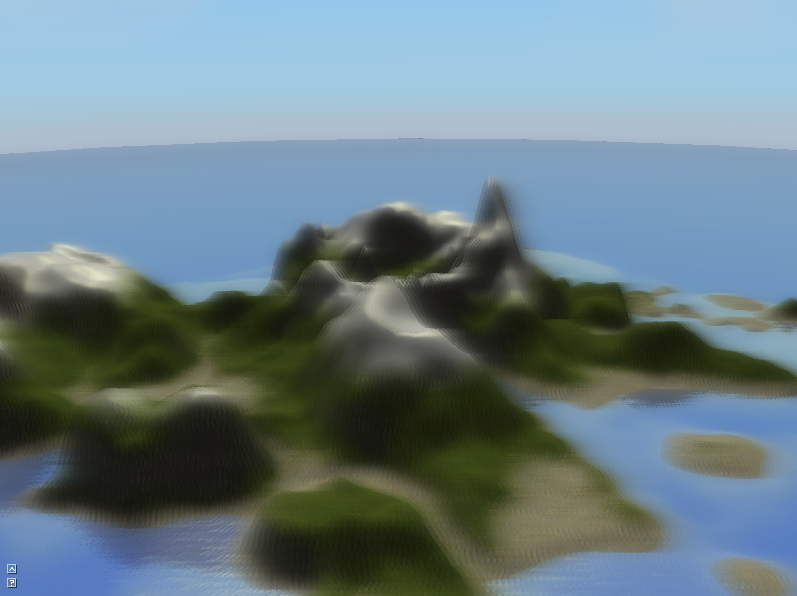
\includegraphics[width=5cm]{motionBlur}
  \caption{Ghosting motion blur using an accumulation texture.}
\end{figure}


\subsection{Glow}

When looking at natural outdoor environments in bright sunlight,
colors seem to blur or smeer together. We would like to reproduce this
effect using a fullscreen glow post process. Initally we created the
effect with just a single shader. This shader first did a box blur on
the surrounding fragments and then blended that result with the
original fragment. This produced the results we where after, but at a
huge performance overhead. The problem was texture lookups. To blur
the surrounding fragments of an $N \times N$ rectangle, we required
$N^2$ texture lookups. We solved this by applying the separable
convolution technique. In the first post process pass a horizontal
blurring is performed, then in the second pass a vertical blurring is
performed on the resulting image of the previous pass and this is then
blended together with the original non-blurred scene. For an $N \times
N$ rectangle we've now reduced $N^2$ texture lookups to $2N$, while
achieving the same effect.

% @TODO show the non blurred + blurred = glow images

As can be seen on \reffig{fig:glow}, a subtle smeering gives a
smoother and more natural looking image. The shader that does the
vertical blurring can be seen in \reflst{lst:glowShader}.

\begin{listing}
\label{lst:glowShader}
\centering
  \lstinputlisting[language=C++]{../data/shaders/glow.frag}
\caption{The vertically blurring glow shader.}
\end{listing}


\subsection{Depth of field}

When filming or photografing through a lens an effect called depth of
field occurs. Essentially everything not in focus by the camera
becomes blurry, and the greater the difference between the object in
focus and the out-of-focus object the more blurry the object will
appear.

With the color texture and depth texture of the rendered scene it is
possible to emulate this effect. In our example the focus of the
camera will always be the center of the screen.

To create the effect we first have to determine how out of focus a
fragment is, which determines teh fragments blurring offset. This is
done by computing the difference between the depth at the center of
the screen and the depth at the fragment.

As before in the glow effect we again create the blur by sampling a
box around the fragment. This time though the distance between sample
points is not constant, but proportional to the blurring offset. The
fragments in focus or near focus have a small blurring offset and thus
won't be much blurred, while fragments with a high blurring offset
will be sampled inside a larger square and thus be blurrier.

Instead of doing a box blur, we decided to blur with a half circle
kernel, as can be seen on \reffig{fig:halfCircle}. To increase
effectivness we tried squaring the error term and came up with the
kernel in \reffig{fig:squaredHalfCircle}, which while faster still
provided a pleasing result.

The result can be seen on \reffig{fig:depthOfField} where hill in the
background and the horizon have been slightly. The shader that creates
the horizontal depth of field blurring can be seen in \reflst{lst:dofShader}.

\begin{figure}
  \label{fig:depthOfField}
  \centering
  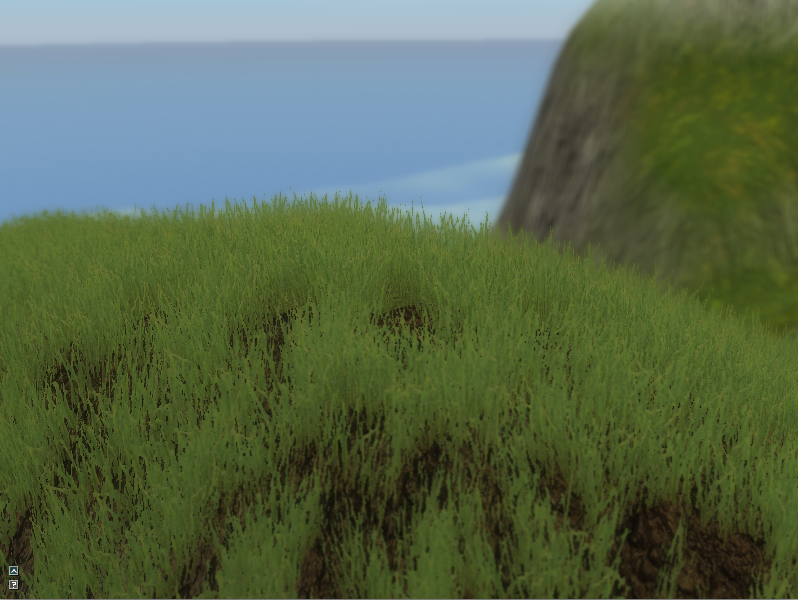
\includegraphics[width=8cm]{depthOfField}
  \caption{The depth of field effect is clearly visible in the background.}
\end{figure}

\begin{listing}
\label{lst:dofShader}
\centering
\lstinputlisting[language=C++]{../data/shaders/HorizontalDepthOfField.frag}
\caption{The horizontal blurring depth of field shader.}
\end{listing}



\subsection{Summary}

Storing and rebinding the previous framebuffer means that we can chain
several post process nodes together to form complex effects or
minimize the cost of applying an effect by using for example separable
convolution.

% One/two fbos pr node is a waste but makes it easy to setup and they
% can be configured individually

% Other effects have been implemented, like wobble, edge detection, pixelate and an underwater that combines...

% Next step is merge



%%% Local Variables:
%%% mode: latex
%%% TeX-master: t
%%% TeX-PDF-mode: t
%%% End:
